\documentclass[12pt,aspectratio=169]{beamer}
\usetheme{metropolis}
\setbeamersize{text margin left=.5cm,text margin right=.5cm}
\usepackage[lf]{carlito}
\usepackage{siunitx}
\usepackage{tikz}
\usepackage{mathpazo}
\usepackage{bm}
\usepackage{mathtools}
\usepackage[ISO]{diffcoeff}
\diffdef{}{ op-symbol=\mathsf{d} }
\usepackage{xcolor,colortbl}

\setmonofont{Ubuntu Mono}
\setlength{\parskip}{0pt}
\renewcommand{\baselinestretch}{1}

\sisetup{
  inter-unit-product=\cdot,
  per-mode=symbol
}

\tikzset{
  >=latex
}

%\newcommand{\iii}{\hat{\bm\imath}}
%\newcommand{\jjj}{\hat{\bm\jmath}}
%\newcommand{\kkk}{\hat{\bm k}}


\title{Class 15: Gauss's Law}
\subtitle{Advanced Placement Physics C}
\author[TML]{Dr.\ Timothy Leung}
\institute{Olympiads School}
\date{Updated: Summer 2022}

\newcommand{\pic}[2]{
  \includegraphics[width=#1\textwidth]{#2}
}
\newcommand{\eq}[2]{
  \vspace{#1}{\Large
    \begin{displaymath}
      #2
    \end{displaymath}
  }
}
%\newcommand{\iii}{\ensuremath\hat{\bm{\imath}}}
%\newcommand{\jjj}{\ensuremath\hat{\bm{\jmath}}}
%\newcommand{\kkk}{\ensuremath\hat{\bm{k}}}
\newcommand{\iii}{\ensuremath\hat\imath}
\newcommand{\jjj}{\ensuremath\hat\jmath}
\newcommand{\kkk}{\ensuremath\hat k}



\begin{document}

\begin{frame}
  \maketitle
\end{frame}


\section{Gauss's Law}

\begin{frame}{Flux}
  \textbf{Flux} is an important concept in many disciplines in physics. The
  flux of a vector quantity $\vec X$ is the amount of that quantity flowing
  through a surface. In integral form:

  \eq{-.2in}{
    \Phi=\int\vec X\cdot\dl\vec A\quad\text{or}\quad
    \Phi=\int(\vec X\cdot\hat n)\dl A
  }

  The direction of the infinitesimal area $\dl\vec A$ is \textbf{outward normal}
  to the surface.
  \begin{center}
    \pic{.3}{eflux}
  \end{center}
\end{frame}



\begin{frame}{Flux}
  \vspace{.2in}$\Phi$ can be something physical, like water, or bananas, or
  something abstract, like electric field (which is what we are interested
  in). We can compute a flux as long as there is a vector field i.e.\
  $\vec X=\vec X(x,y,z)$. In the case of \textbf{electric flux}, the quantity
  $\vec X$ is just the
  electric field, i.e.:
    
  \eq{-.1in}{
    \boxed{ \Phi_E=\int\vec E\cdot\dl\vec A }
  }
  \begin{center}
    \pic{.3}{eflux}
  \end{center}
\end{frame}



\begin{frame}{Electric Flux and Gauss's Law}
  \textbf{Gauss's law} tells us that if we have a closed surface (think of
  the surface of a balloon), the total electric flux is very well defined:

  \eq{-.1in}{
    \boxed{
      \Phi_E=\oint\vec E\cdot\dl\vec A=\frac{Q_\text{encl}}{\epsilon_0}
    }
  }
    
  where
  \begin{itemize}
  \item $Q_\text{encl}$ is the charge enclosed by the surface
  \item $\epsilon_0=\SI{8.85e-12}{C^2/N.m^2}$ is the permittivity of free space
  \end{itemize}
  That closed surface is called a \textbf{Gaussian surface}
\end{frame}



\begin{frame}{Closed Surfaces}
  \begin{columns}
    \column{.55\textwidth}
    A \textbf{closed surface} is one that does not have a boundary, like the
    sphere, toroid, and cube on the left.
    \column{.45\textwidth}
    \pic1{800px-SurfacesWithAndWithoutBoundary}
  \end{columns}
\end{frame}



\begin{frame}{Electric Field from a Positive Point Charge}
  \begin{columns}
    \column{.35\textwidth}
    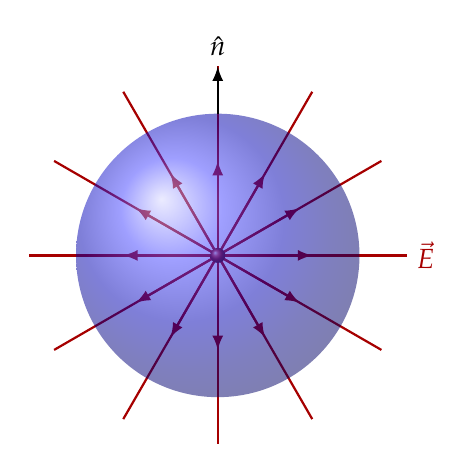
\begin{tikzpicture}[scale=1.2]
      \foreach \x in {1,...,12}{
        \draw[red!65!black,thick,rotate=30*\x,->](0,0)--(0,1);
        \draw[red!65!black,thick,rotate=30*\x](0,0)--(0,2);
      }
      \shade[ball color=red!70!black] circle(.08);
      \node[red!65!black,right] at (2,0) (E) {$\vec E$};
      \uncover<2>{
        \shade[ball color=blue,opacity=.5] circle(1.5);
        \draw[thick,->](0,1.5)--(0,2) node[above]{$\hat n$};
      }
    \end{tikzpicture}
    
    \column{.65\textwidth}
    By symmetry, electric field lines must be radially outward from the charge,
    so the integral reduces to:

    \eq{-.1in}{
      \Phi_E=\oint\vec E\cdot\dl\vec A=EA=\frac q{\epsilon_0}
    }

    Since area of a sphere is $A=4\pi r^2$, we recover Coulomb's law and the
    magnitude of the electric field from a point charge:

    \eq{-.1in}{
      E=\frac1{4\pi\epsilon_0}\frac q{r^2}=\frac{kq}{r^2}
    }
  \end{columns}
\end{frame}



\begin{frame}{Uniformly-Charged Thin Shell}
  For a uniformly-charged spherical thin shell with radius $R$ and a total
  charge of $Q$.
  
  \vspace{.1in}
  \begin{columns}
    \column{.28\textwidth}
    \centering
    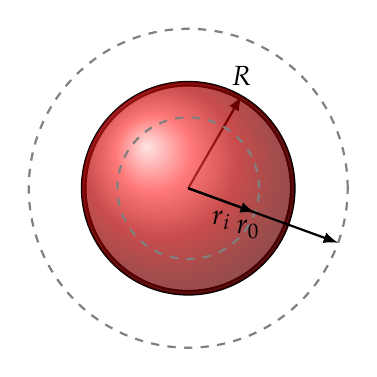
\begin{tikzpicture}[scale=.9]
      \draw[thick,fill=black!70] circle(1.5);
      \draw[thick,fill=white] circle(1.45);
      \draw[thick,->,rotate=60](0,0)--(1.5,0)node[above]{$R$};
      \uncover<1>{
        \shade[ball color=red,opacity=.7] circle(1.5);
      }
      \uncover<2>{
        \draw[thick,->,rotate=-20](0,0)--(1,0)node[midway,below]{$r_i$};
        \draw[dashed,gray,thick] circle(1);
      }

      \uncover<3>{
        \draw[thick,->,rotate=-20](0,0)--(2.25,0)node[pos=.4,below]{$r_0$};
        \draw[dashed,gray,thick] circle(2.25);
      }
    \end{tikzpicture}
    
    \column{.72\textwidth}

    \uncover<2->{
      Inside the shell ($r_i<R$), there is no enclosed charge, therefore
      the electric field must be zero:
      
      \eq{-.1in}{
        \oint\vec E\cdot\dl\vec A=\frac{q_\text{encl}}{\epsilon_0}=0
        \quad\rightarrow\quad E=0
      }
    }

    \uncover<3>{
      Outside the shell ($r_0>R$), the enclosed charge is
      $Q$, and the electric field is given by the same equation as the point
      charge:
      
      \eq{-.15in}{
        \oint\vec E\cdot\dl\vec A=\frac Q{\epsilon_0}
        \;\rightarrow\; E=\frac Q{\epsilon_0A}
        =\frac1{4\pi\epsilon_0}\left[\frac Q{r^2}\right]
      }
    }
  \end{columns}
\end{frame}



\begin{frame}{Uniformly-Charged Thin Shell}
  The electric field strength $E$ can be plotted as a function of the distance
  $r$ from the center of the shell:
  \begin{center}
    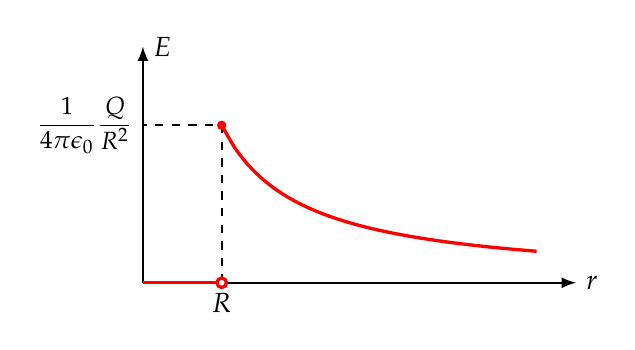
\begin{tikzpicture}
      \draw[thick,->](0,0)--(0,3)  node[right]{$E$};
      \draw[thick,->](0,0)--(5.5,0)node[right]{$r$};
      \draw[thick,dashed](1,0)
      --(1,2) node[pos=0,below]{$R$}
      --(0,2) node[left]{\small$\dfrac1{4\pi\epsilon_0}\dfrac Q{R^2}$};
      \draw[very thick,red,smooth,domain=1:5] plot(\x,{2/\x});
      \draw[very thick,red](0,0)--(1,0);
      \draw[very thick,red,fill=white](1,0) circle(.06);
      \fill[red](1,2) circle(.06);
    \end{tikzpicture}
  \end{center}
  \begin{itemize}
  \item This graph may be familiar because the graph for the gravitational field
    strength inside a uniform shell is exactly the same
  \item For gravity, replace $\epsilon_0$ with $4\pi G$
  \end{itemize}
\end{frame}



%\begin{frame}{Worksheet Examples}
%  Follow the worksheet for these examples:
%  \begin{itemize}
%  \item Uniformly-charged sphere
%  \item Charged sphere with variable charge density
%  \item Infinitely-long charge rod with uniform density
%  \end{itemize}
%\end{frame}



\begin{frame}{Electric Field Near an Infinite Plane of Charge}
  \begin{columns}
    \column{.25\textwidth}
    \pic{1.1}{elec_gauss_figure9}

    \column{.75\textwidth}
    \begin{itemize}
    \item Charge density (charge per unit area) $\sigma$
    \item By symmetry, $\vec E$ must be perpendicular to the plane
    \item Our Gaussian surface is a cylinder shown in the left with an area
      $A$; the height of the cylinder is unimportant
    \item Nothing ``flows out'' of the side of the cylinder, only at the ends
    \item The total flux is $\Phi_E=E(2A)$
    \item The enclosed charge is $Q_\text{encl}=\sigma A$
    \end{itemize}
  \end{columns}
\end{frame}



\begin{frame}{Electric Field Near an Infinite Plane of Charge}
  \begin{columns}
    \column{.27\textwidth}
    \pic1{elec_gauss_figure9}

    \column{.73\textwidth}
    Gauss's law simplifies to:
    
    \eq{-.1in}{
      \oint\vec E\cdot\dl\vec A=\frac{q_\text{encl}}{\epsilon_0}
      \;\rightarrow\;
      E(2A)=\frac{\sigma A}{\epsilon_0}
    }

    Solving for $E$, we get:

    \eq{-.1in}{
      \boxed{E=\frac\sigma{2\epsilon_0}}
    }
    \begin{itemize}
    \item $E$ is a constant
    \item Independent of distance from the plane
    \item Both sides of the plane are the same
    \end{itemize}
  \end{columns}
\end{frame}



\begin{frame}{Electric Field Between Parallel Charged Plates}
  \begin{center}
    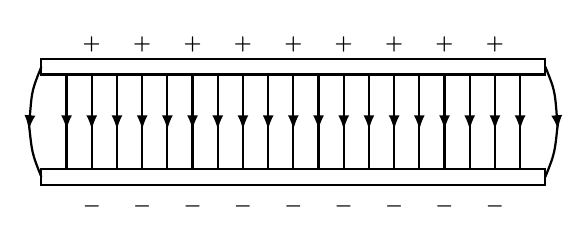
\begin{tikzpicture}[xscale=.8]
      \begin{scope}[thick]
        \draw(0,0) rectangle (8,.2);
        \draw(0,1.4) rectangle (8,1.6);
        \foreach \x in {.4,.8,1.2,...,7.6}{
          \draw[->](\x,1.4)--(\x,.7);
          \draw    (\x,1.4)--(\x,.2);
        }
        \foreach \x in {.8,1.6,2.4,...,7.2}{
          \node at (\x,1.78) {\scriptsize $\bm{+}$};
          \node at (\x,-.28) {\scriptsize $\bm{-}$};
        }
        
        \draw[->] (0,1.5)..controls(-.15,1.2)..(-.2,.7);
        \draw (-.2,.8)..controls(-.15,.4)..(0,.1);
        
        \draw[->](8,1.5)..controls(8.15,1.2)..(8.2,.7);
        \draw    (8.2,.8)..controls(8.15,.4)..(8,.1);
      \end{scope}
    \end{tikzpicture}
  \end{center}
  \begin{itemize}
  \item Two plates, each producing an electric field pointing in
    the same direction
  \item The total electric field is twice the value of \emph{one} infinite
    plane, pointing from the positively charged plate toward the negatively
    charged plate

    \eq{-.2in}{
      \boxed{E=\frac\sigma{\epsilon_0}}
    }
  \item $\vec E$ outside the plates is very low (close to zero), except for
    fringe effects at the edges of the plates
  \end{itemize}
\end{frame}



\begin{frame}{Electric Field and Electric Potential Difference}
  Recall the relationship between electric field ($\vec E$) and electric
  potential difference ($V$):
    
  \eq{-.1in}{
    \vec E=-\diffp Vr\hat r
  }
  
  This relationship holds regardless of the charge configuration.
\end{frame}




\begin{frame}{Electric Field and Electric Potential Difference}
  \begin{center}
    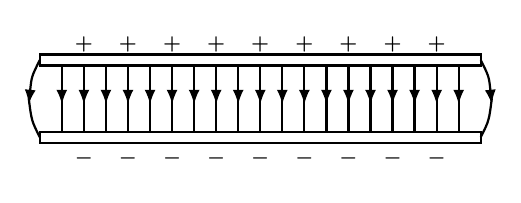
\begin{tikzpicture}[scale=.7]
      \begin{scope}[thick]
        \draw(0,0) rectangle (8,.2);
        \draw(0,1.4) rectangle (8,1.6);
        \foreach\x in {.4,.8,1.2,...,7.6}{
          \draw[->](\x,1.4)--(\x,.7);
          \draw(\x,1.4)--(\x,.2);
        }
        \foreach\x in {.8,1.6,2.4,...,7.2}{
          \node at (\x,1.78) {\scriptsize $\bm{+}$};
          \node at (\x,-.28) {\scriptsize $\bm{-}$};
        }
        
        \draw[->](0,1.5)..controls(-.15,1.2)..(-.2,.7);
        \draw(-.2,.8)..controls(-.15,.4)..(0,.1);
        
        \draw[->](8,1.5)..controls(8.15,1.2)..(8.2,.7);
        \draw(8.2,.8)..controls(8.15,.4)..(8,.1);
      \end{scope}
    \end{tikzpicture}
  \end{center}
  In the case of two parallel plates, the electric field is uniform, and the
  relationship simplifies to:

  \eq{-.2in}{
    \boxed{E=\frac{\Delta V}d}
  }
  \begin{center}
    \begin{tabular}{l|c|c}
      \rowcolor{pink}
      \textbf{Quantity} & \textbf{Symbol} & \textbf{SI Unit} \\ \hline
      Electric field intensity & $E$ & \si{\newton\per\coulomb}\\
      Potential difference between plates & $\Delta V$ & \si\volt \\
      Distance between plates       & $d$ & \si\metre
    \end{tabular}
  \end{center}
\end{frame}
\end{document}
